% !TEX root = ../thesis.tex
% [H] means put the figure HERE, directly when you input this code.
% Remove this to let LaTeX place the figure where it decides is best
\begin{figure}[H]
% \begin{figure}
	\centering
	
% We use a figure width of 48.5% of the width of one line of text on 
% the page so there is some space between the images.
	\subfloat[Inaccurate GenAI image from the system.]{
		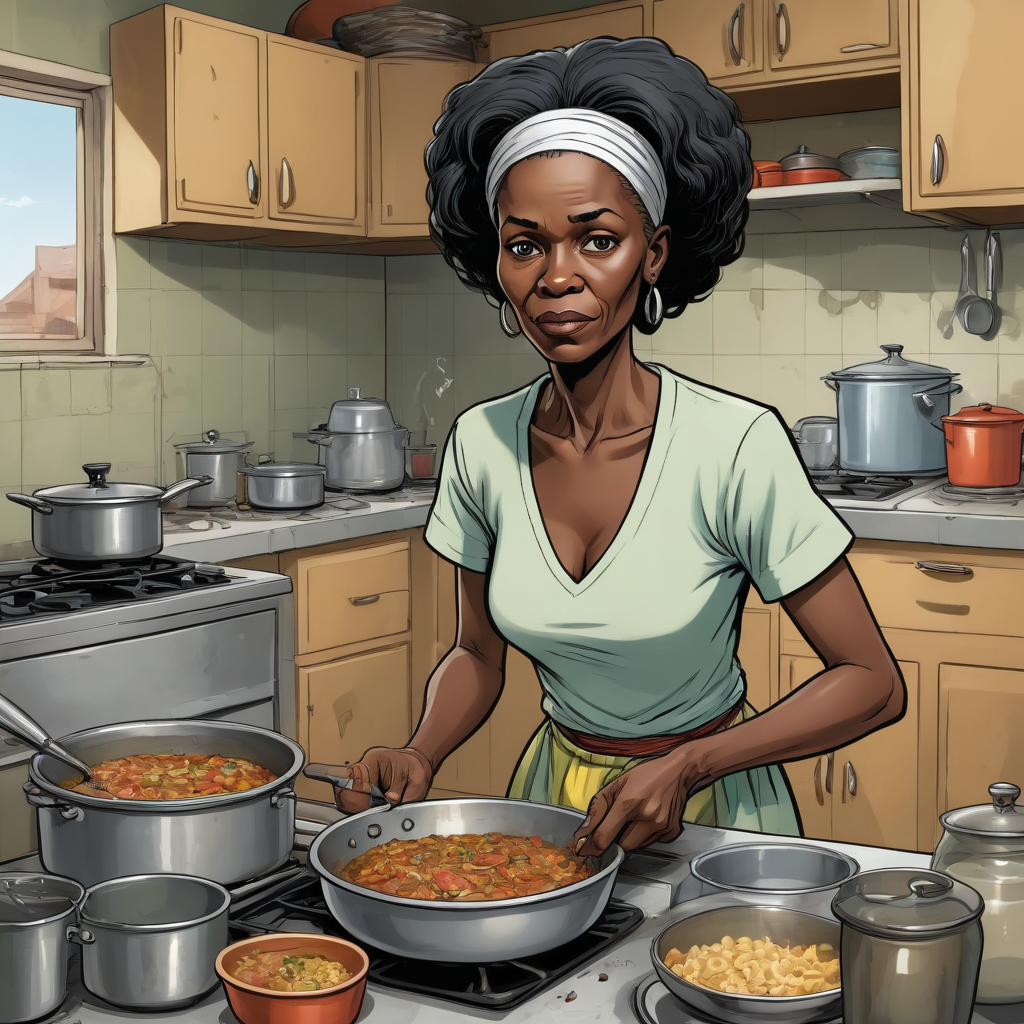
\includegraphics[width=0.485\textwidth]{graphics/c_cook1.png}\label{fig:example_2x1_a}
	}\hfill % Spacing between sub-figures displayed next to each other.
	\subfloat[Accurate GenAI image from personal investigation.]{
		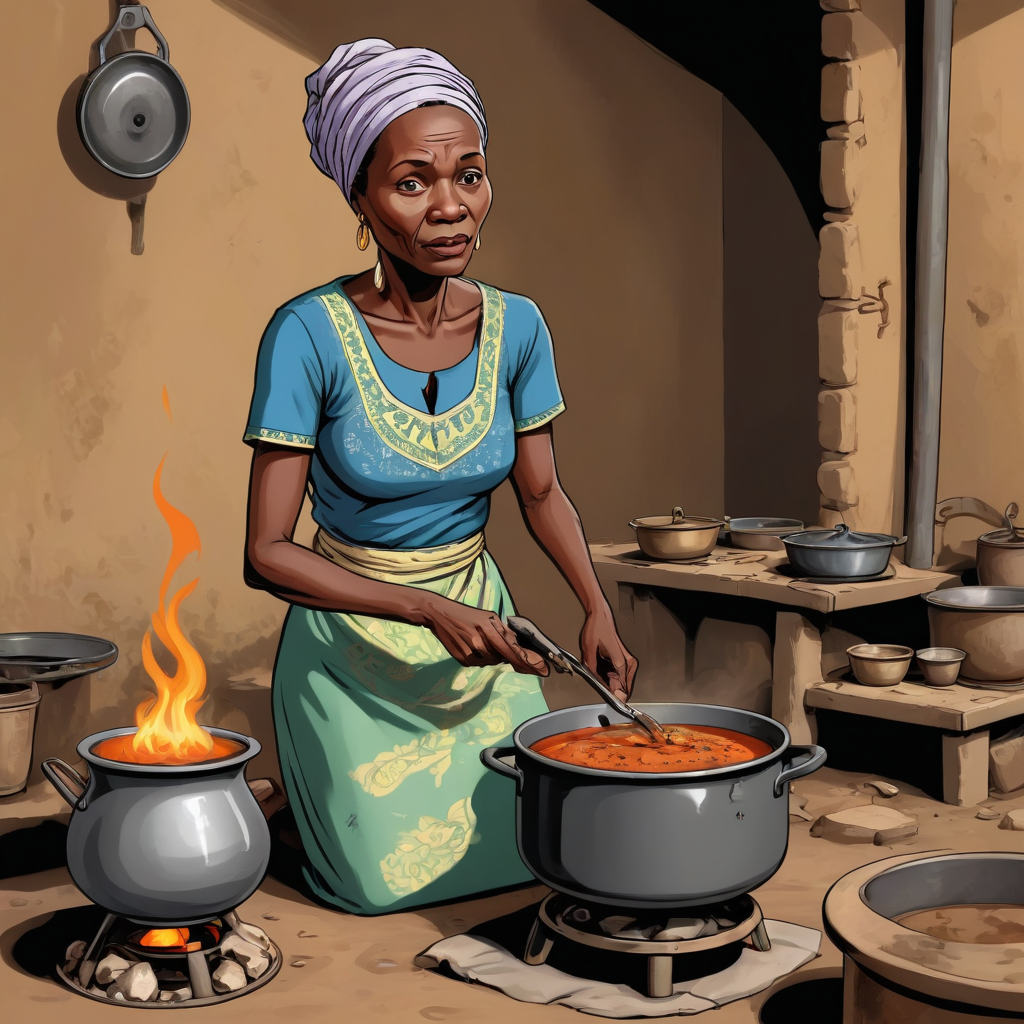
\includegraphics[width=0.485\textwidth]{graphics/c_cook2.png}\label{fig:example_2x1_b}
	}\\ % New line before caption.

% Caption is defined with a short and long version. The short version is shown in the 
% List of Figures section, and the long version is used directly with the figure. 	
	\caption[Images showing a woman in her "small slum kitchen"]{
Images showing a woman in her "small slum kitchen".
	
% Figure labels should be defined at the end of the caption to ensure proper numbering.
	\label{fig:food_2x1}
	}
	
\end{figure}